\documentclass{standalone}
\usepackage{mintikz}

\usepackage{xfp}

\begin{document}
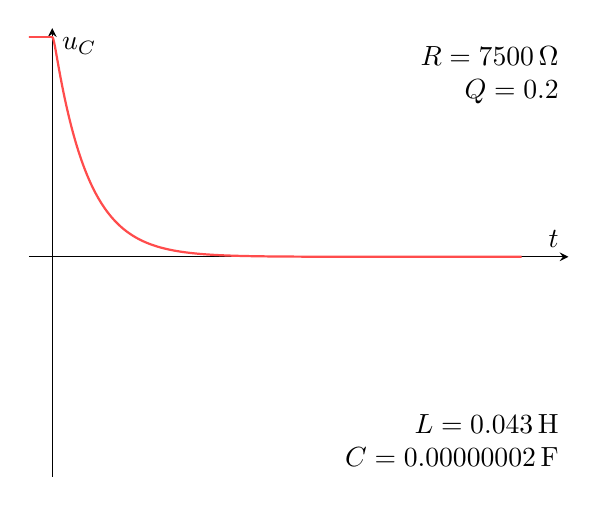
\begin{tikzpicture}[]
    \def\E{5}
    \def\R{7500}
    \def\L{0.043}
    \def\C{0.00000002}
    \def\Q{(1/\R)*sqrt(\L/\C)}
    \def\Qeff{\fpeval{\Q}}
    \def\wo{sqrt(1/(\L*\C))}
    \def\w{\wo*sqrt(1-1/(4*\Q^2))}
    \def\xmax{2.2e-3}
    \def\rp{-(\wo/(2*\Q))+\wo*sqrt(1/(4*\Qeff^2)-1)}
    \def\rpeff{\fpeval{\rp}}
    \def\rl{-(\wo/(2*\Q))-\wo*sqrt(1/(4*\Qeff^2)-1)}
    \def\rleff{\fpeval{\rl}}
    \def\rdif{\fpeval{\rpeff-\rleff}}
    \begin{axis}[
        xmin=-1e-4, xmax=2.2e-3,
        ymin=-5, ymax=5.2,
        xlabel=$t$, ylabel=$u_C$,
        axis lines=center,
        xtick=\empty, ytick=\empty,
        clip=false]
        \addplot[thick,
        domain=-1e-4:0,
        samples=500,
        Red!70]
        {\E};
        \addplot[thick,
        domain=0:0.002,
        samples=500,
        Red!70]
        {(\E/(\rdif))*(\rpeff*exp(\rleff*\x)-\rleff*exp(\rpeff*\x))};
        \node[anchor=north east, align=right] (RQtext) at (axis cs: \xmax, 5) {
                $R = \R\,\Omega$\\
                $Q = \fpeval{round(\Q,2)}$
        };
        \node[anchor=south east, align=right] (LCtext) at (axis cs: \xmax,-5) {
                $L = \L\,\rm H$\\
                $C = \C\,\rm F$
        };
    \end{axis}
\end{tikzpicture}
\end{document}
